%
% teil1.tex
%
% (c) 2023 Vincent Haufe, Hochschule Rapperswil
%
% !TEX root = ../../buch.tex
% !TEX encoding = UTF-8

\section{Motivation
\label{mellin:section:teil1}}
\rhead{Motivation}

Folgendes Kapitel orientiert sich zu Beginn stark am Kapitel 2 von 
\cite{mellin:mendezmueller-book}.
\smallskip

Es sei folgendes Registrierungsproblem gegeben: Wir haben zwei Funktionen 
$f(x)$ und $g(x)$, welche bis auf eine Verschiebung identisch sind 
(siehe Abb. \ref{fig:mellin:f1}).
Dieses einfache Beispiel mit eindimensionalen Funktionen soll symbolisch 
für das Problem gelten, in der Bildverarbeitung könnten dies gegeneinander 
verschobene Bilder sein, die zur Deckung gebracht werden sollen, das 
Prinzip bleibt hierbei dasselbe.
\begin{figure}
    \centering
    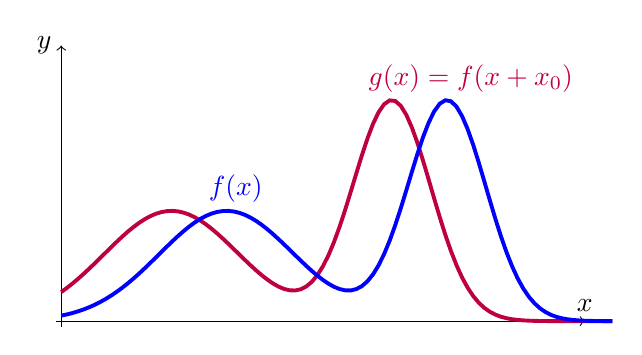
\begin{tikzpicture}[scale=0.70]
    \draw[->] (-0.1,0) -- (9.5,0) coordinate[label={$x$}];
    \draw[->] (0,-0.1) -- (0,5) coordinate[label={left:$y$}];
    \node at (5.4,4.4) [right, color=purple] {$\displaystyle g(x) = f(x + x_0)$};
    \node at (2.5,2.4) [right, color=blue] {$\displaystyle f(x)$};
    \draw[color=purple,line width=1.4pt]
    plot[domain=0:{10},samples=100]
    ({\x},{4*(exp(-(\x-2-4)^2) + 0.5 * exp(-(\x+2-4)^2/3))});
    \draw[color=blue,line width=1.4pt]
    plot[domain=0:{10},samples=100]
    ({\x},{4*(exp(-(\x-2-5)^2) + 0.5 * exp(-(\x+2-5)^2/3))});
    \end{tikzpicture}
    \caption{Gegeneinander verschobene Funktionen
    \label{fig:mellin:f1}}
\end{figure}

Die Aufgabe besteht nun darin, bei gegebenen Funktionen $f(x)$ und $g(x)$ 
die unbekannte Verschiebung $x_0$ zu ermitteln. 
Ein mathematisch naheliegender Ansatz ist das Standard-Skalarprodukt 
\footnote{Siehe auch Kapitel \ref{buch:chapter:skalarprodukte}}, 
welches ein quantitatives Mass für die Ähnlichkeit zweier Funktionen 
liefert \footnote{Anmerkung: Die beiden Funktionen müssen so geschaffen 
sein, dass das Skalarprodukt konvergiert}.
\begin{equation}
    \langle f,g \rangle 
    = \int \overline{f(x)} \cdot g(x) \,\mathrm{d}x
    \label{mellin:skalaprodukt}
\end{equation}
Der Wert den das Skalarprodukt liefert ist genau dann am grössten, wenn die 
beiden Funktionen identisch sind.
Wir lassen also eine Verschiebung der zweiten Funktion zu und ermitteln, 
für welche Verschiebung das Skalarprodukt maximal wird.
Dies führt auf die Kreuzkorrelation
\begin{equation}
    (f \star g)(\tau) 
    = \int_\mathbb{R} f(x) \cdot g(x-\tau)\,\mathrm{d}x,
    \label{mellin:kreuzkorrelation+}
\end{equation}
die selber eine Funktion der Verschiebung $\tau$ ist. 
Wenn $\tau =  x_0$ liegen die ursprünglichen Funktionen exakt übereinander 
da
% \begin{proof}
%     \begin{equation}
%         g(x)
%         = f(x + x_0)
%         g(x - \tau)
%         = f(x + x_0 - \tau) = f(x)
%     \end{equation}
% \end{proof}
$g(x) = f(x + x_0)$ und $g(x - \tau) = f(x + x_0 - \tau) = f(x)$ für 
$\tau =  x_0$ und die Kreuzkorrelation ist maximal. 
Mathematisch ausgedrückt findet sich $x_0$ mit
\begin{equation}
    x_0 = 
    \argmax\limits_{\tau \in \mathbb{R}}{(f \star g)(\tau)}
    .
    \label{mellin:x0}
\end{equation}
Die Kreuzkorrelation führt zum Erfolg, ist aber, sofern sie sich nicht 
analytisch berechnen lässt (in Anwendungen generell nicht der Fall) eine 
ziemlich rudimentäre Methode, die mit sehr grossem Rechenaufwand verbunden 
ist, da für jeden Wert der Verschiebung $\tau$ ein Integral berechnet 
werden soll.
Die effizientere Lösung bietet die Fouriertheorie.

Durch Spiegeln von $g(x) \rightarrow \check{g}(x)$ verwandelt sich die 
Korrelation in eine \emph{Faltung}.
Das Faltungstheorem der Fouriertheorie lässt uns aus der Faltung im 
Ortsraum eine Multiplikation im Frequenzraum machen.
Die Fouriertransformierte der gespiegelten Funktion 
$\check{g}(x) = {g}(-x)$ ist dabei die konjugiert-komplexe 
Fouriertransformierte von $g(x)$:
$\overline{\mathcal{F}\{g \}} = \overline{\hat{g}(\omega)}$.
Der Faltungssatz auf die Korrelation angewendet lautet also
\begin{equation}
    \mathcal{F}\{(f \star g)\} 
    = \mathcal{F}\{f \} \cdot \overline{\mathcal{F}\{g \}}
\end{equation}
und somit findet sich die Lösung nach \eqref{mellin:x0}
\begin{equation}
    x_0 = 
    \argmax\limits_{x \in \mathbb{R}}
    {\mathcal{F}^{-1}(\hat{f}(\omega) \cdot \overline{\hat{g}(\omega)})}
    \label{mellin:x0ft}
\end{equation}
Diese Methode funktioniert deshalb, da die Hin- und Rücktransformationen 
zahlreicher bekannten Funktionen gut untersucht sind. 
Viele Standardfunktionen sind tabelliert und mathematische Software bieten 
ausgefeilte Methoden zur schnellen und effizienten Berechnung der 
Transformationspaare. 


\subsection{Registrierungsproblem für skalierte Funktionen
\label{mellin:subsection:regskal}}
Wie im ersten Beispiel gezeigt lässt sich jenes Registrierungsproblem 
mithilfe der Fouriertransformation elegant lösen.
Dies hat deshalb funktioniert, weil das gestellte Problem eine 
Verschiebung beinhaltete, also eine Addition im Argument, die der 
Gruppenoperation der Fouriertransformation entspricht und somit 
automatisch auf die ``normale'' Faltung der additiven reellen 
Gruppe $(\mathbb{R},+)$ geführt hat. 
Als nächstes wollen wir eine Variante dieses Registrierungsproblems 
betrachten, die uns auf eine andere Korrelation und somit einer leicht 
anderen Faltungsformel führt.

Wieder haben wir zwei Funktion $f(x)$ und $g(x)$, die zur Deckung gebracht 
werden sollen. Dieses mal unterscheiden sie sich nur 
über einen positiven \emph{Skalierungsfaktor} $s \in \mathbb{R^+}$ im 
Argument gemäss Abbildung \ref{fig:mellin:f2}.
\begin{figure}
    \centering
    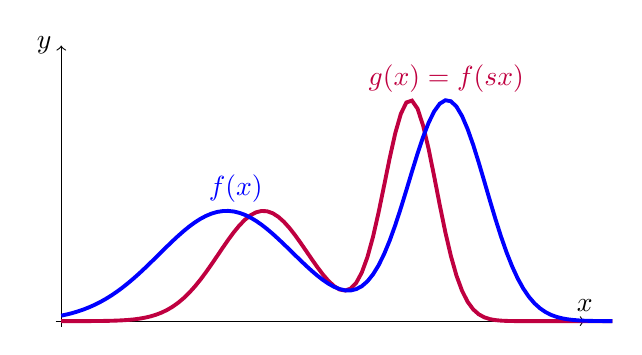
\begin{tikzpicture}[scale=0.70]
    \draw[->] (-0.1,0) -- (9.5,0) coordinate[label={$x$}];
    \draw[->] (0,-0.1) -- (0,5) coordinate[label={left:$y$}];
    \node at (5.4,4.4) [right, color=purple] {$\displaystyle g(x) = f(sx)$};
    \node at (2.5,2.4) [right, color=blue] {$\displaystyle f(x)$};
    \draw[color=purple,line width=1.4pt]
    plot[domain=0:{10},samples=100]
    ({\x},{4*(exp(-((\x-5)*1.5-2)^2) + 0.5 * exp(-((\x-5)*1.5+2)^2/3))});
    \draw[color=blue,line width=1.4pt]
    plot[domain=0:{10},samples=100]
    ({\x},{4*(exp(-(\x-2-5)^2) + 0.5 * exp(-(\x+2-5)^2/3))});
    \end{tikzpicture}
    \caption{Gegeneinander skalierte Funktionen
    \label{fig:mellin:f2}}
\end{figure}
Das Vorgehen verläuft nun analog zum ersten Beispiel. Wir lassen eine 
Skalierung von $g(x)$ so zu, dass für den richtigen Wert von
$\sigma$, der ursprüngliche Skalierungsunterschied der Funktionen genau 
aufgehoben wird und das Skalarprodukt
\begin{equation}
    k(\sigma) 
    = \int_\mathbb{R^+} f(x) \cdot g(\sigma^{-1} \cdot x)\,\mathrm{d}x
    \label{mellin:ksigma}
\end{equation}
maximal wird.
Die Funktion $k(\sigma)$ wirkt wie eine Kreuzkorrelation auf der 
multiplikativen Gruppe der positiven reellen Zahlen $(\mathbb{R^+},\cdot)$, 
jedoch fehlt dafür noch eine kleine Anpassung der Formel, auf die später 
eingengangen werden soll. 
Wieder könnte man das Integral für verschiedene Werte von $\sigma$ 
numerisch auswerten und so den richtigen Faktor zu finden. 
Da dies aber die gleichen Probleme wie vorher beinhaltet, drängt sich die 
Frage auf, lässt sich die Lösung auch hier über Fourieranalyse finden?